\documentclass[a4paper,11pt]{article} 
\usepackage[francais]{babel}
\usepackage[T1]{fontenc} 
\usepackage[utf8]{inputenc} 
\usepackage{graphicx}
\usepackage{color}
\usepackage{hyperref}
\usepackage{bookmark}
\usepackage{array}
\usepackage{geometry}
\geometry{a4paper, margin=1in}

\begin{document}

\begin{figure}

\includegraphics[width=0.3\textwidth]{images/logolemansU.png}
\hspace{150pt} 
\includegraphics[width=0.3\textwidth]{images/logo_ic2.png} 
\end{figure}

\title{\textbf{\color{blue} Le Mans Université}\color{black}
\\ Licence Informatique \textit{3ème année}
\\ Module IHM
\\ \textit{Plateforme de suivi et d’actualités sur les crypto-monnaies}
\\ \textbf{Personas}}
\author{LEPINE François\\BORRY Lenny\\GHRIB Yacine\\VEAU-BIGOT Damien}
\date{\today} 
\maketitle 
\newpage

\tableofcontents
\newpage

\section{Introduction}
Un persona est une représentation fictive et détaillée d'un utilisateur ou client type, basée sur des données réelles, des recherches et des hypothèses éclairées.

\subsection{Description détaillée}
\noindent Description type:
\begin{itemize}
    \item \textbf{Nom:} Un nom fictif pour le rendre plus humain.
    \item \textbf{Données démographiques:} Âge, sexe, localisation, statut familial, etc.
    \item \textbf{Occupation et situation professionnelle:}  Rôle, niveau d'expérience, secteur d'activité.
    \item \textbf{Besoins et objectifs:} Ce que l'utilisateur souhaite accomplir.
    \item \textbf{Frustrations et points de douleur:} Ce qui complique leur vie ou leur expérience.
    \item \textbf{Comportements et préférences:} Comment ils interagissent avec des produits, services ou technologies.
\end{itemize}

\section{Personas}

\subsection{Persona - TYPE 1}
\begin{minipage}{0.6\textwidth} % 60% de la largeur pour le texte
    \textbf{Nom:} Dimitri Mpondo-Guibert.\\
    \textbf{Âge:} 34 ans.\\
    \textbf{Situation:} En couple.\\
    \textbf{Profession:} Développeur blockchain.\\
    \textbf{Statut familial:} Vit avec sa compagne et leur chat.\\
    \textbf{Besoins et objectifs:} Recherche des outils précis pour suivre l’évolution des cours des crypto-monnaies qu’il utilise dans ses projets. Il souhaite avoir des alertes sur les mouvements importants des prix.\\
    \textbf{Frustrations et points de douleur:} Perte de temps à consulter plusieurs sites pour les graphiques et les actualités.\\
\end{minipage}%
\hspace{1cm}
\begin{minipage}{0.3\textwidth} % 30% de la largeur pour l'image
    \begin{center}
        
\includegraphics[width=\textwidth]{images/Dimitri.jpeg} % Remplacer 'image.jpeg' par le chemin de votre image
    \end{center}
\end{minipage}

\subsection{Persona - TYPE 2}
\begin{minipage}{0.6\textwidth} % 60% de la largeur pour le texte
    \textbf{Nom:} Julie Martin.\\
    \textbf{Âge:} 27 ans.\\
    \textbf{Situation:} Célibataire.\\
    \textbf{Profession:} Étudiante en finance.\\
    \textbf{Statut familial:} Vit seule dans un studio.\\
    \textbf{Besoins et objectifs:} S’informe sur les fondamentaux des crypto-monnaies et cherche à comprendre les tendances de marché pour ses cours d’analyse financière.\\
    \textbf{Frustrations et points de douleur:} A du mal à trouver des ressources claires et fiables dans l’océan d’informations disponibles en ligne.\\
\end{minipage}%
\hspace{1cm}
\begin{minipage}{0.3\textwidth} % 30% de la largeur pour l'image
    \begin{center}
        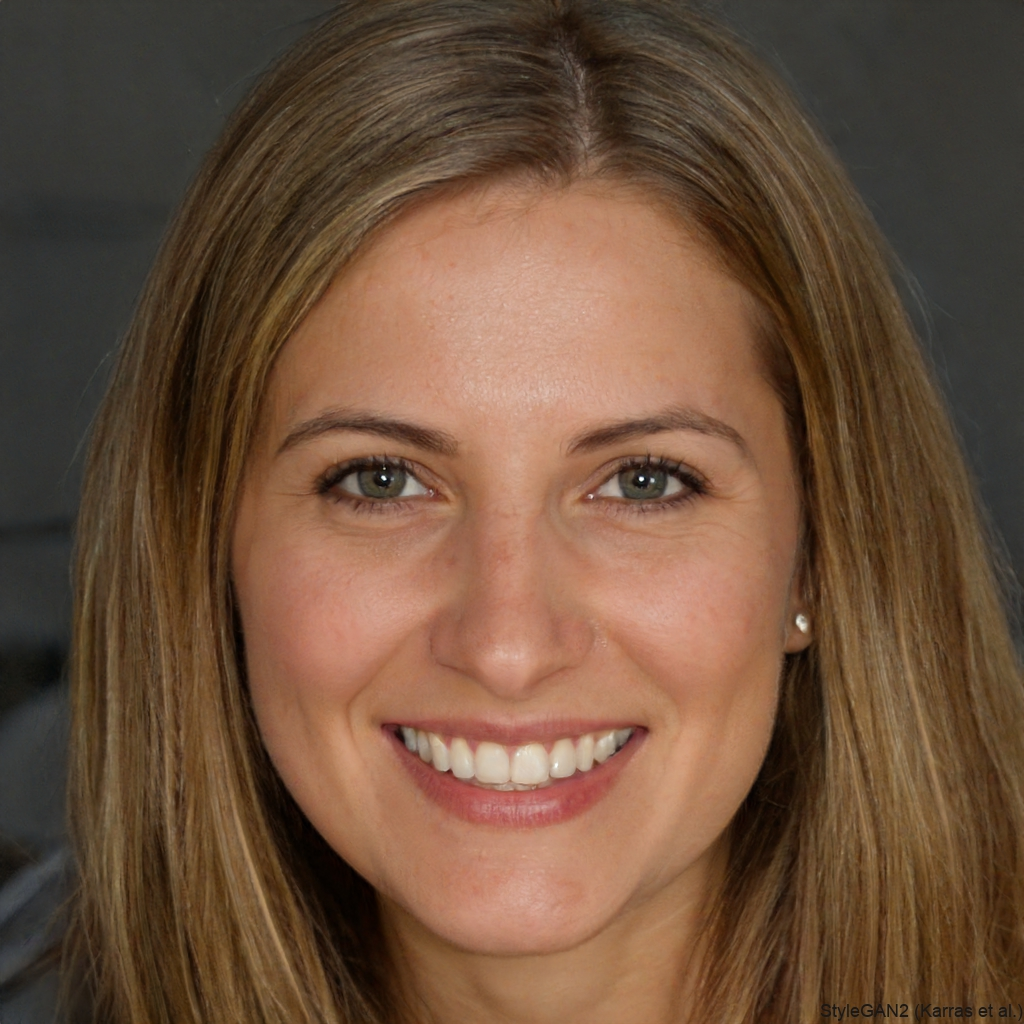
\includegraphics[width=\textwidth]{images/camelott.jpeg} % Remplacer 'image.jpeg' par le chemin de votre image
    \end{center}
\end{minipage}

\subsection{Persona - TYPE 3}
\begin{minipage}{0.6\textwidth} % 60% de la largeur pour le texte
\textbf{Nom:} Apu Kumar.\\
\textbf{Âge:} 32 ans.\\
\textbf{Situation:} Marié.\\
\textbf{Profession:} Consultant en investissement.\\
\textbf{Statut familial:} Père de deux enfants.\\
\textbf{Besoins et objectifs:} Cherche à diversifier ses portefeuilles clients avec des crypto-monnaies. Besoin de suivre les actualités économiques et les évolutions réglementaires du secteur.\\
\textbf{Frustrations et points de douleur:} Difficulté à repérer rapidement les crypto-monnaies émergentes ayant un potentiel.\\
\end{minipage}%
\hspace{1cm}
\begin{minipage}{0.3\textwidth} % 30% de la largeur pour l'image
    \begin{center}
        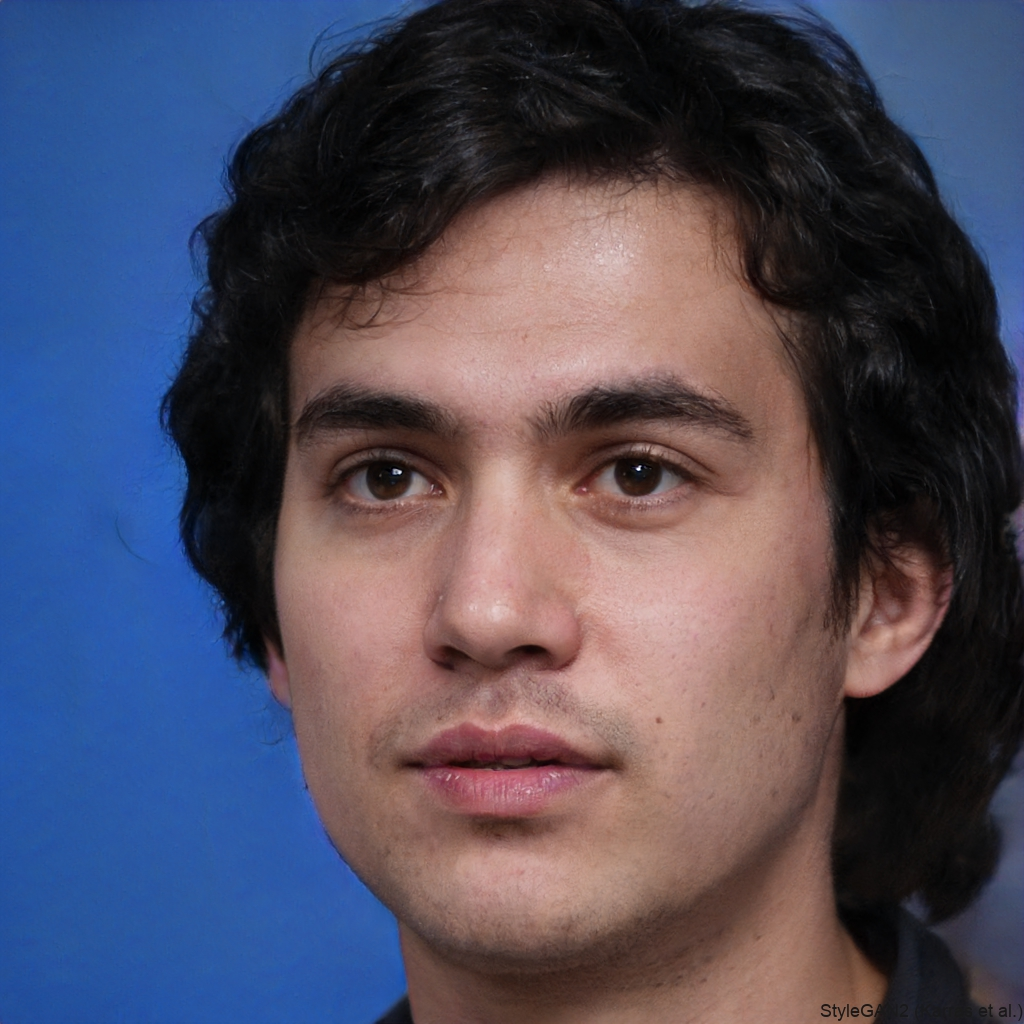
\includegraphics[width=\textwidth]{images/crypto-expert.jpeg} % Remplacer 'image.jpeg' par le chemin de votre image
    \end{center}
\end{minipage}

\subsection{Persona - TYPE 4}
\begin{minipage}{0.6\textwidth} % 60% de la largeur pour le texte
\textbf{Nom:} Laura Duval.\\
\textbf{Âge:} 21 ans.\\
\textbf{Situation:} Étudiante.\\
\textbf{Profession:} Participe à des projets NFT en tant que créatrice.\\
\textbf{Statut familial:} Vit en colocation avec trois amis.\\
\textbf{Besoins et objectifs:} Veut suivre les tendances des cryptos associées aux NFT pour optimiser son travail et anticiper les hausses de popularité.\\
\textbf{Frustrations et points de douleur:} Les informations sur les NFT et les cryptos sont souvent éclatées sur des plateformes différentes.\\
\end{minipage}%
\hspace{1cm}
\begin{minipage}{0.3\textwidth} % 30% de la largeur pour l'image
    \begin{center}
        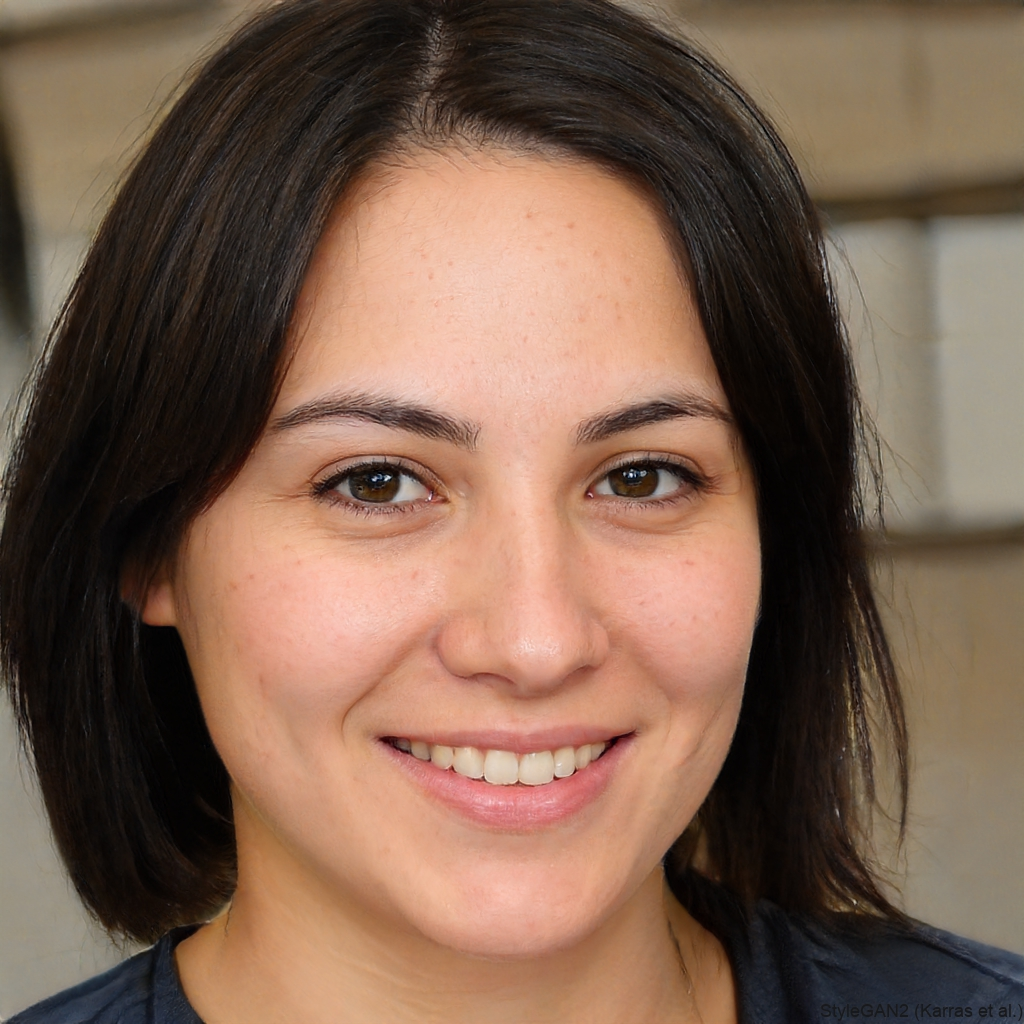
\includegraphics[width=\textwidth]{images/etudiante.jpeg} % Remplacer 'image.jpeg' par le chemin de votre image
    \end{center}
\end{minipage}

\subsection{Persona - TYPE 5}
\begin{minipage}{0.6\textwidth} % 60% de la largeur pour le texte
\textbf{Nom:} François Dubois.\\
\textbf{Âge:} 56 ans.\\
\textbf{Situation:} Retraité.\\
\textbf{Profession:} Ancien directeur marketing.\\
\textbf{Statut familial:} Marié, ses enfants ont quitté le foyer.\\
\textbf{Besoins et objectifs:} Passionné par l’économie, il s’intéresse aux crypto-monnaies pour compléter son épargne retraite et suivre les tendances.\\
\textbf{Frustrations et points de douleur:} Manque d’expérience technique avec les plateformes modernes et les graphiques complexes.\\
\end{minipage}%
\hspace{1cm}
\begin{minipage}{0.3\textwidth} % 30% de la largeur pour l'image
    \begin{center}
        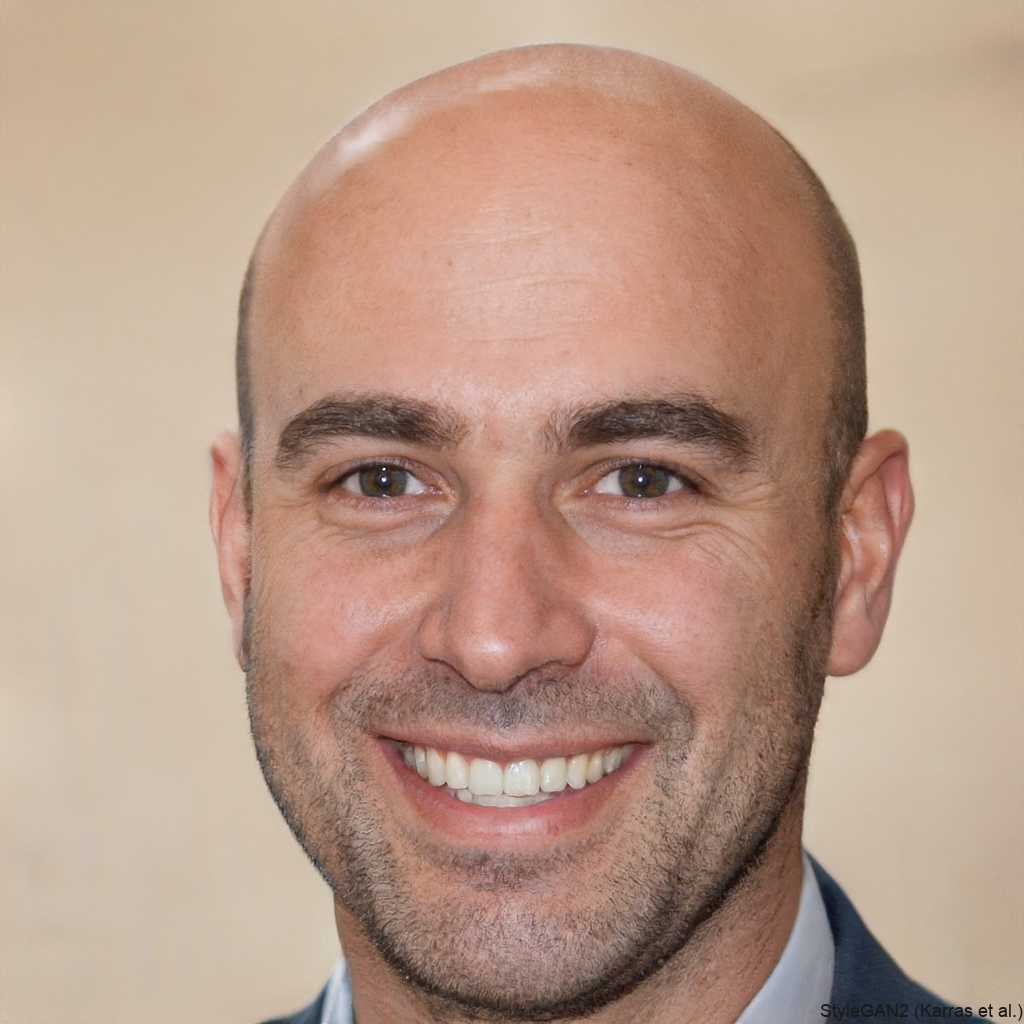
\includegraphics[width=\textwidth]{images/francois_50_ans.jpeg} % Remplacer 'image.jpeg' par le chemin de votre image
    \end{center}
\end{minipage}

\end{document}

